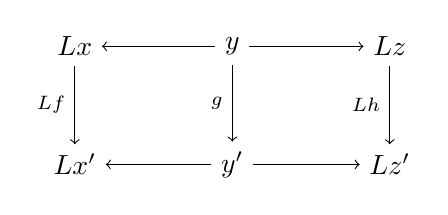
\begin{tikzpicture}
\node (v2) at (-5.5,5) {$Lx$};
\node (v1) at (-3.5,5) {$y$};
\node (v3) at (-1.5,5) {$Lz$};
\node (v5) at (-5.5,3.5) {$Lx'$};
\node (v4) at (-3.5,3.5) {$y'$};
\node (v6) at (-1.5,3.5) {$Lz'$};
\draw [->] (v1) edge (v2);
\draw [->] (v1) edge (v3);
\draw [->] (v4) edge (v5);
\draw [->] (v4) edge (v6);
\draw [->] (v2) edge
	node [left] {\scriptsize $Lf$} (v5);
\draw [->] (v1) edge 
	node [left] {\scriptsize $g$} (v4);
\draw [->] (v3) edge
	node [left] {\scriptsize $Lh$} (v6);
\end{tikzpicture}